%% Introduction
\section{Methods}
\subsection{Feedforward ANC using FXLMS}
%The adaptive feedforward ANC system is shown on \autoref{fig:ANCFeedforward}


The system in \autoref{fig:ANCFeedforward} outputs a control signal $y[n]$, which ideally is a counter-phase signal of the noise. The counter-phase signal is generated by inputting the reference signal $x[n]$ into a control filter consisting of adaptive coefficients $\bar{b}$ representing the inverse of the transfer function from the reference microphone to the headphone loudspeaker. This means that the signal $y[n]$ is the inverse of x[n]. The coefficients are adapted using the FXLMS algorithm. This adaption ensures that the optimum counter-phase signal is outputtet even if the transfer function changes e.g changing angle of incident. The FXLMS algorithm inputs the filtered reference $f[n]$ signal along with the error signal $e[n]$. The filtered reference signal is used combined with the error signal to determine new optimal coefficients for the control filter, this is shown in equation \ref{eq:FXLMS}. The signals from (1)(3) are converted to the digital domain using an ADC and anti aliasing filters (AA) before processing. When processed, the output $y[n]$ is reconstructed and converted using a DAC.


\begin{figure}[H]
	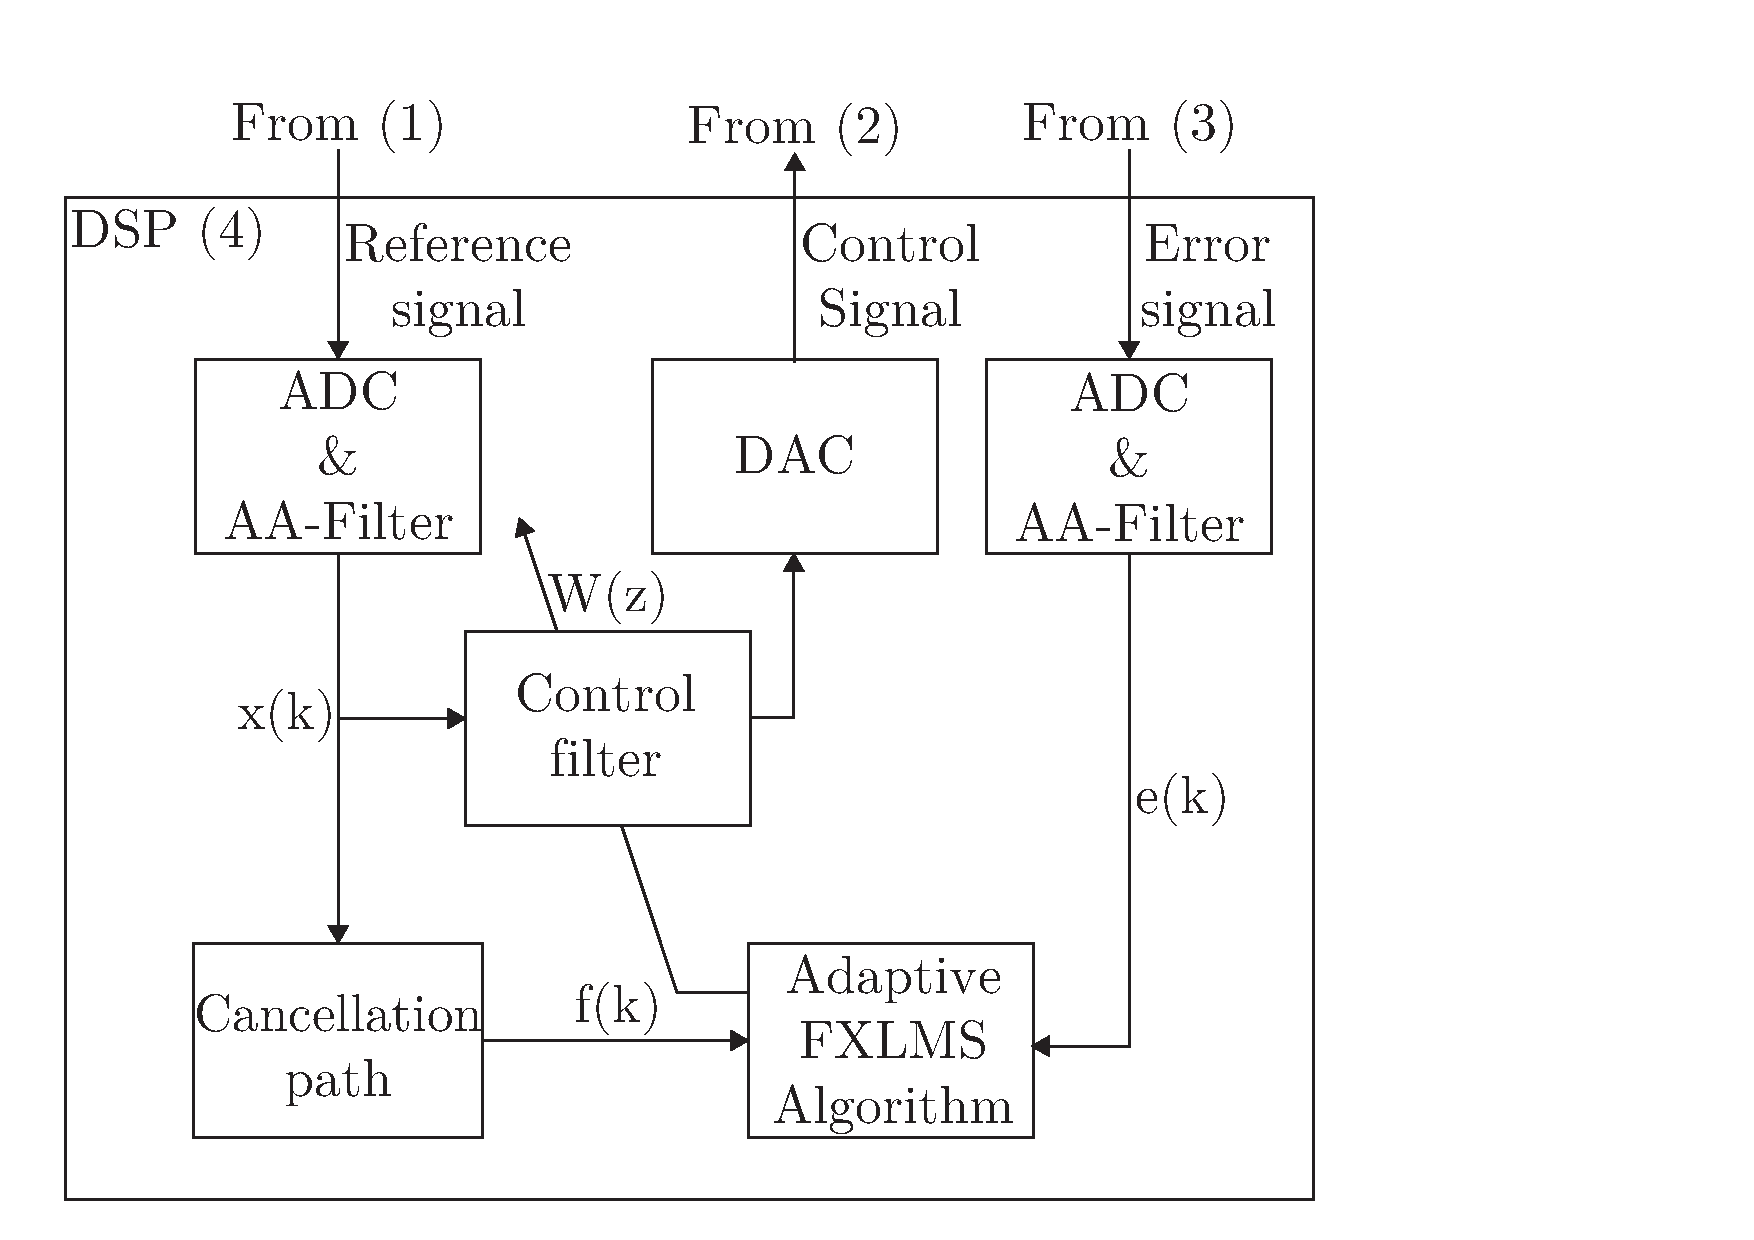
\includegraphics[width=1\columnwidth]{figures/ArticleIllustrations/ANCFeedForward}
	\caption{Adaptive feedforward ANC system.}
	\label{fig:ANCFeedforward}
\end{figure}

%\begin{figure}[H]
%	\centering
%	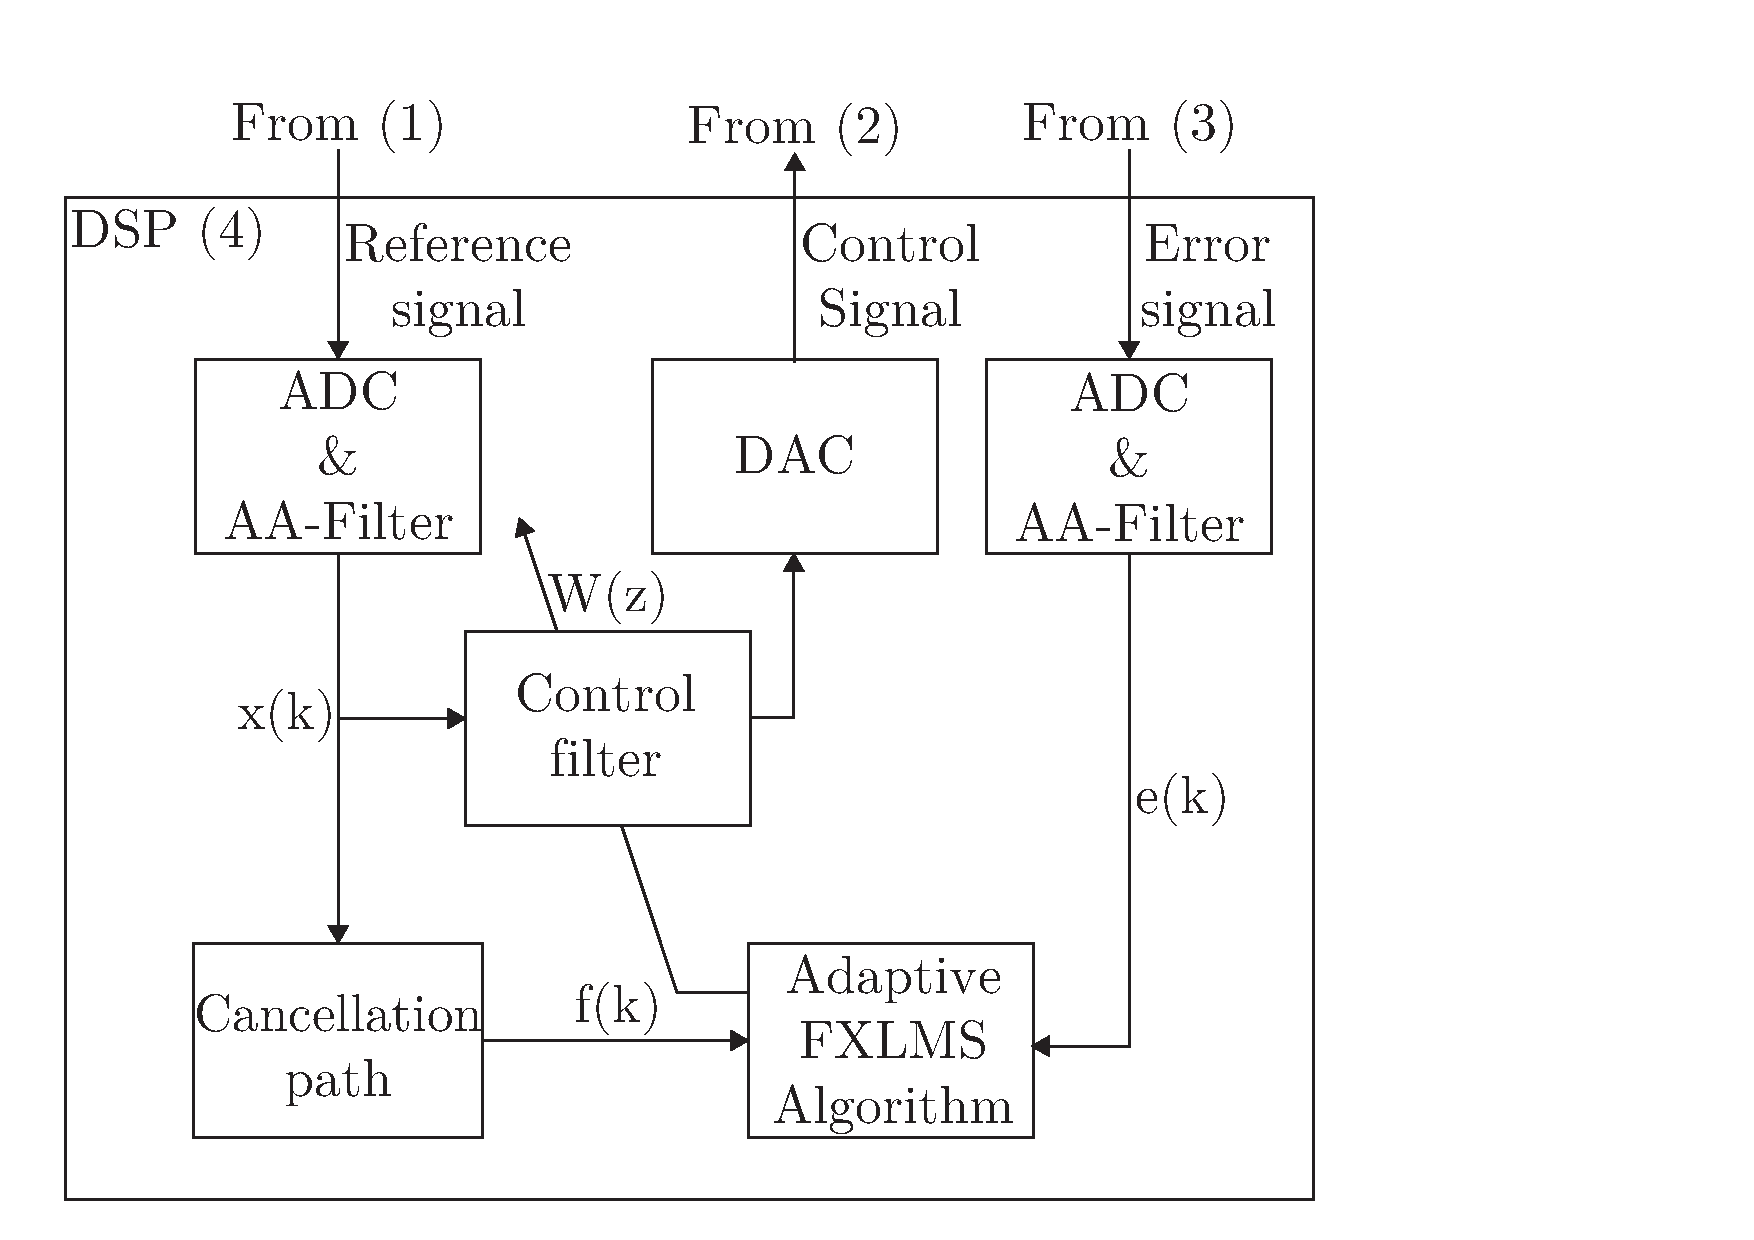
\includegraphics[width=1\columnwidth]{figures/ArticleIllustrations/ANCFeedForward}
%	\caption{Adaptive feedforward ANC system}
%	\label{fig:ANCFeedforward}
%\end{figure}


\textbf{Control Filter}, shown in \autoref{eq:Output}, is initialized with the inverse of the measured impulse response of the represented transfer function. An order of 256 taps is chosen based on subjective testing in simulation.
\vspace{-3mm} % yeah I know - Sorry Mikkel!
\begin{equation}\label{eq:Output}
y[n]=\sum_{j=0}^{L-1}b_j[n]x[n-j]
\end{equation}
where $b_j[n]$ is the weight coefficients written as  $b[n]=[b_0[n],b_1[n], \cdots, b_{L-1}[n]]^T$.
\\\\
\textbf{FXLMS} is the optimization algorithm which updates the control filter coefficients using the FXLMS method shown in \autoref{eq:FXLMS}.
\begin{equation}\label{eq:FXLMS}
b_j[n+1] = b_j[n] - 2\mu e[n]f[n-j]
\end{equation}
where $\mu$ is the convergence factor, $e[n]$ is the error and $f[n]$ is the reference convolved with the Cancellation Path.
\\\\
\textbf{Cancellation Path} (CP) shown in \autoref{eq:CP}.
\begin{equation}\label{eq:CP}
f[n]=\sum_{j=0}^{L-1}c_jx[n-j]
\end{equation}
where $c_j$ is the coefficient of a measured transfer-function from the headphone loudspeaker to the error microphone in the ear of a Head and Torso Simulator (HATS). In the literature \cite{Hansen} the CP is adaptively adjusted, but it is assumed constant because the position of the headphone does not change while measured on a HATS. This assumption is made because it is irrelevant for verifying if LP is a plausible solution. 


%When implementing the system, delays exist due to the anti-aliasing and reconstruction filters. The delays of the system exceeds the propagation time of sound from the reference microphone to the headphone loudspeaker resulting in poor performance. Therefore an LP-algorithm is proposed to predict future samples in order to decrease the effect of the time delays.

\subsection{Characteristics of Speech}
Speech can be split into two main classes, voiced and unvoiced. Voiced sounds are characterized by a strong periodicity, with the fundamental frequency referred to as the pitch frequency (50 - 500 Hz). Unvoiced sounds are characterized as random. Speech is a non stationary signal and can only be assumed Wide Sense Stationary (WSS) for periods of 20 - 30 ms \cite{Speech}. 

\subsection{Linear Prediction of Speech}
The outlines of the prediction system is shown in figure \ref{fig:LinearPredictionOverview}. The system predicts $\hat{x}[n+P]$ by utilizing adaptive linear prediction coefficients (LPCs) $\hat{\bar{a}}$, in a Wiener filter, determined using a framebased Auto Correlation Function (ACF) $\hat{r}_x[l]$ \cite{LinearPrediction}.   

\begin{figure}[H]
	\centering
	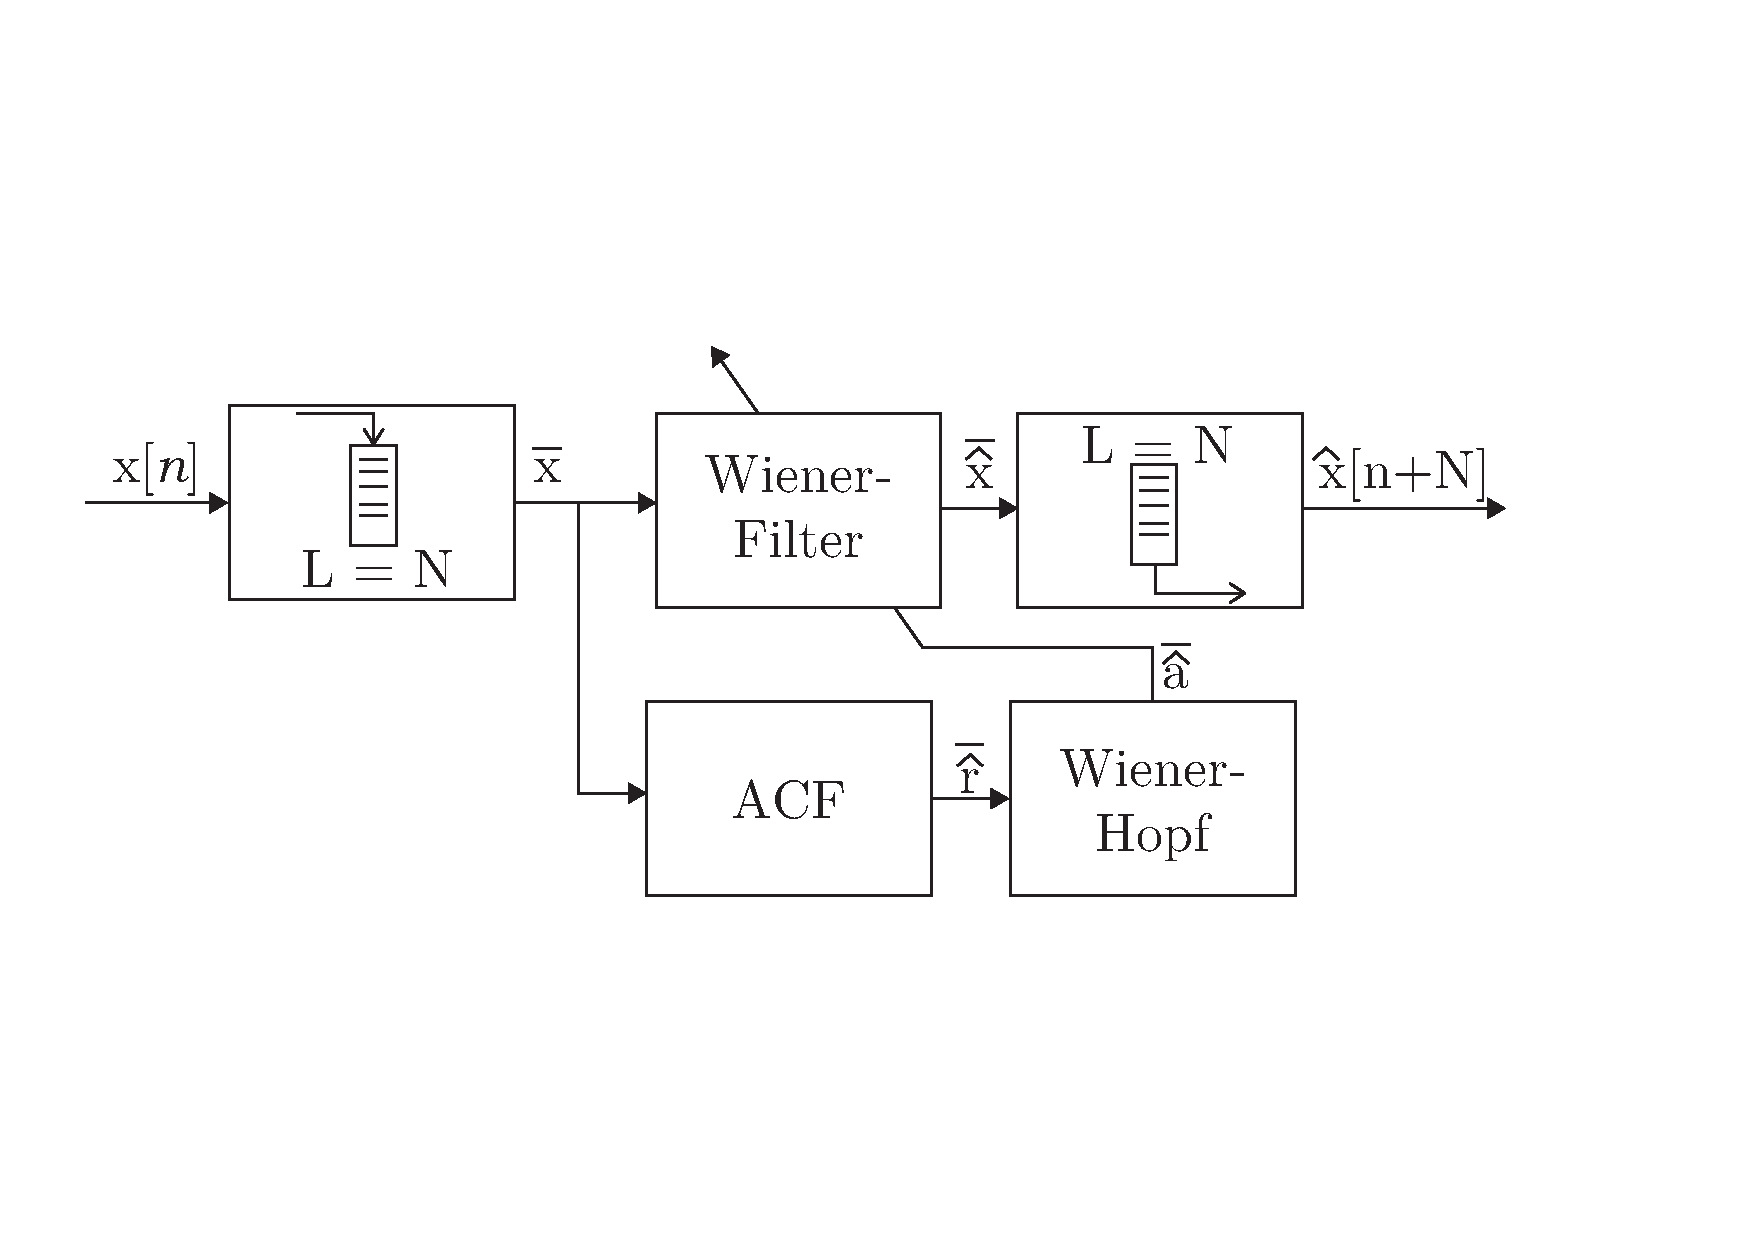
\includegraphics[width=\columnwidth]{figures/ArticleIllustrations/WienerHopf}
	\caption{Linear prediction system.}
	\label{fig:LinearPredictionOverview}
\end{figure}


The ACF is estimated by nonrecursive estimation, shown in \autoref{eq:nonrecursive}, with framelength N. The nonrecursive estimation relies on a well defined window in order to increase the periodicity of the ACF. This is done by weighting the center of the frame highest, assuming highest periodicity in the center of a frame. Therefore a Hamming window ($w$) is applied being one of the most widely used. Furthermore overlapping ($O$) can be used to increase the update rate of the ACF without having a small framelength.  
\begin{equation}\label{eq:nonrecursive}
%%r_x[l,m] = \sum^{m}_{n=m-N+1+\left| l\right|} x_l[n]w_l[m-n]
\hat{r}_x[l] = \sum^{N}_{n=\left| l\right|} x_l[n]w_l[N-n]
\end{equation}
%\begin{multline}\label{eq:nonrecursive}
%R[l,m] = \sum^{m}_{n=m-N+1+\left| l\right|} \\ x[n]w[m-n] x[n-\left| l\right|]w[m-n+\left| l\right|]
%\end{multline}
%\begin{equation}
%R[l,m]=\sum^{m}_{n=m-N+1+\left| l\right|}x[n]w[m-n] x[n-\left| l\right|]w[m-n+\left| l\right|]
%\end{equation}
where $x_l[n]=x[n]x[n-l]$, $w_l[n]=w[n]w[n+l]$ and $l$ is the lag. The LPCs are determined using \autoref{eq:normal}, known as the Wiener-Hopf equation.
\begin{equation}\label{eq:normal}
\hat{R}  \bar{a} = -\bar{\hat{r}}_x
\end{equation}
where $\hat{R}$ is the covariance matrix $\hat{C}_{xx}$, $\bar{\hat{a}}$ is the LPCs $\bar{\hat{a}} = [\hat{a}_0 , \hat{a}_1, \cdots, \hat{a}_{N-1}]^T$ and $\bar{\hat{r}}_x$ is the ACF, $\bar{\hat{r}}_x = [\hat{r}_x[1] , \hat{r}_x[2], \cdots, \hat{r}_x[N]]^T$. \autoref{eq:normal} can be rewritten as shown in \autoref{eq:normal2} yielding the LPCs directly.  
 \begin{equation}\label{eq:normal2}
\bar{\hat{a}} = \hat{-R^{-1}} \bar{\hat{r}}_x
\end{equation}
Calculating $\hat{R^{-1}}$ is computationally heavy on a DSP. Therefore to estimate the LPCs the Levinson-Durbin method is used \cite{LinearPrediction}. Prediction using Wiener filtering, shown in equation \ref{eq:Predictor}, can then be applied to the current frame for prediction of the next frame. To decrease the computational load $M$ LPCs should be used. 

\begin{equation}\label{eq:Predictor}
\hat{x}[n+p] =- \sum^{M-1}_{i=1}\hat{a}_i[n]x[(n+p)-i]
\end{equation}

Using equation \ref{eq:Predictor} in cascade where $\hat{x}[n+2]$ is estimated using $\hat{x}[n+1]$ and $x[n]$ up until $\hat{x}[n+P]$. 

\subsection{Determining System Parameters}
The parameters which should be detemined are $fs$, $N$, $O$, $M$ and $P$. fs is determined   


\begin{figure}[H]
	\centering
	\textbf{\textit{Here is going to be a graph of PG determined by fs}}
	\caption{PG }
	\label{fig:fsPredict}
\end{figure}


These are detemined respectively using a Prediction Gain ($PG$) to find the optimum value. The PG is defined in \autoref{eq:PG}. 
\begin{equation}\label{eq:PG}
PG = 10 log_{10}\bigg(\frac{\sigma^2_x}{\sigma^2_\varepsilon}\bigg) = 10 log_{10}\bigg(\frac{E\{x^2[n]\}}{E\{\varepsilon^2[n]\}}\bigg)
\end{equation}
where PG is the ratio between the variance of the input signal $x[n]$ and the variance of the prediction error $\varepsilon$ in (dB). The higher the PG the better the prediction is. The PG of variable $N$, $O$ and $M$ is seen on \autoref{fig:PredictParameters}. 
\begin{figure}[H]
	\centering
	\textbf{\textit{Here is going to be a graph of PG determined by N}}
	\textbf{\textit{Here is going to be a graph of PG determined by O}}
	\textbf{\textit{Here is going to be a graph of PG determined by M}}
	\caption{PG }
	\label{fig:PredictParameters}
\end{figure}

The determination of the parameters are choosen based on having the largest PG with the lowest value of $N$, $O$ and $M$. $N$ is determined to be 500, $O$ is determined to be 300 and $M$ is determined to be 50. These values will be used in the predictor.

\subsection{Feedforward LP FXLMS}
The adaptive ANC system combined with the predictor is shown on \autoref{fig:LPFXLMS}. Here the predictor will be inserted before the ANC system. The predictor need to compensate for both the ADC delay and the DAC delay, which are assumed to have the same delay. Therefore the predictor needs to predict $880$ $\mu s$ out which is equvialent to 42 samples with fs equal to 48000 Hz.      

\begin{figure}[H]
	\centering
	\textbf{\textit{Here is going to be a figure showing the combined system}}
	\caption{Combined system}
	\label{fig:LPFXLMS}
\end{figure}

The adaptive ANC will input both the predicted input $\hat{x}[n+P]$ and the measured input $x[n]$.  

\begin{equation}\label{eq:ControlExpanded}
y[n+P]=\sum^{P-1}_{j=0}b_j[n]\hat{x}[(n+P)-j]+\sum^{L-1}_{j=P}b_j[n]x[(n+P)-j]
\end{equation}

\begin{equation}\label{eq:CPExpanded}
f[n+P]=\sum^{P-1}_{j=0}c_j\hat{x}[(n+P)-j]+\sum^{L-1}_{j=P}c_jx[(n+P)-j]
\end{equation}